\documentclass[twoside]{book}

% Packages required by doxygen
\usepackage{calc}
\usepackage{doxygen}
\usepackage{graphicx}
\usepackage[utf8]{inputenc}
\usepackage{makeidx}
\usepackage{multicol}
\usepackage{multirow}
\usepackage{textcomp}
\usepackage[table]{xcolor}

% Font selection
\usepackage[T1]{fontenc}
\usepackage{mathptmx}
\usepackage[scaled=.90]{helvet}
\usepackage{courier}
\usepackage{amssymb}
\usepackage{sectsty}
\renewcommand{\familydefault}{\sfdefault}
\allsectionsfont{%
  \fontseries{bc}\selectfont%
  \color{darkgray}%
}
\renewcommand{\DoxyLabelFont}{%
  \fontseries{bc}\selectfont%
  \color{darkgray}%
}

% Page & text layout
\usepackage{geometry}
\geometry{%
  a4paper,%
  top=2.5cm,%
  bottom=2.5cm,%
  left=2.5cm,%
  right=2.5cm%
}
\tolerance=750
\hfuzz=15pt
\hbadness=750
\setlength{\emergencystretch}{15pt}
\setlength{\parindent}{0cm}
\setlength{\parskip}{0.2cm}
\makeatletter
\renewcommand{\paragraph}{%
  \@startsection{paragraph}{4}{0ex}{-1.0ex}{1.0ex}{%
    \normalfont\normalsize\bfseries\SS@parafont%
  }%
}
\renewcommand{\subparagraph}{%
  \@startsection{subparagraph}{5}{0ex}{-1.0ex}{1.0ex}{%
    \normalfont\normalsize\bfseries\SS@subparafont%
  }%
}
\makeatother

% Headers & footers
\usepackage{fancyhdr}
\pagestyle{fancyplain}
\fancyhead[LE]{\fancyplain{}{\bfseries\thepage}}
\fancyhead[CE]{\fancyplain{}{}}
\fancyhead[RE]{\fancyplain{}{\bfseries\leftmark}}
\fancyhead[LO]{\fancyplain{}{\bfseries\rightmark}}
\fancyhead[CO]{\fancyplain{}{}}
\fancyhead[RO]{\fancyplain{}{\bfseries\thepage}}
\fancyfoot[LE]{\fancyplain{}{}}
\fancyfoot[CE]{\fancyplain{}{}}
\fancyfoot[RE]{\fancyplain{}{\bfseries\scriptsize Generated on Thu Jul 24 2014 15\-:32\-:09 for My Project by Doxygen }}
\fancyfoot[LO]{\fancyplain{}{\bfseries\scriptsize Generated on Thu Jul 24 2014 15\-:32\-:09 for My Project by Doxygen }}
\fancyfoot[CO]{\fancyplain{}{}}
\fancyfoot[RO]{\fancyplain{}{}}
\renewcommand{\footrulewidth}{0.4pt}
\renewcommand{\chaptermark}[1]{%
  \markboth{#1}{}%
}
\renewcommand{\sectionmark}[1]{%
  \markright{\thesection\ #1}%
}

% Indices & bibliography
\usepackage{natbib}
\usepackage[titles]{tocloft}
\setcounter{tocdepth}{3}
\setcounter{secnumdepth}{5}
\makeindex

% Hyperlinks (required, but should be loaded last)
\usepackage{ifpdf}
\ifpdf
  \usepackage[pdftex,pagebackref=true]{hyperref}
\else
  \usepackage[ps2pdf,pagebackref=true]{hyperref}
\fi
\hypersetup{%
  colorlinks=true,%
  linkcolor=blue,%
  citecolor=blue,%
  unicode%
}

% Custom commands
\newcommand{\clearemptydoublepage}{%
  \newpage{\pagestyle{empty}\cleardoublepage}%
}


%===== C O N T E N T S =====

\begin{document}

% Titlepage & ToC
\hypersetup{pageanchor=false}
\pagenumbering{roman}
\begin{titlepage}
\vspace*{7cm}
\begin{center}%
{\Large My Project }\\
\vspace*{1cm}
{\large Generated by Doxygen 1.8.6}\\
\vspace*{0.5cm}
{\small Thu Jul 24 2014 15:32:09}\\
\end{center}
\end{titlepage}
\clearemptydoublepage
\tableofcontents
\clearemptydoublepage
\pagenumbering{arabic}
\hypersetup{pageanchor=true}

%--- Begin generated contents ---
\chapter{Hierarchical Index}
\section{Class Hierarchy}
This inheritance list is sorted roughly, but not completely, alphabetically\-:\begin{DoxyCompactList}
\item Model\begin{DoxyCompactList}
\item \contentsline{section}{librehatti.\-catalog.\-models.\-Attributes}{\pageref{classlibrehatti_1_1catalog_1_1models_1_1Attributes}}{}
\item \contentsline{section}{librehatti.\-catalog.\-models.\-Catalog}{\pageref{classlibrehatti_1_1catalog_1_1models_1_1Catalog}}{}
\item \contentsline{section}{librehatti.\-catalog.\-models.\-Category}{\pageref{classlibrehatti_1_1catalog_1_1models_1_1Category}}{}
\item \contentsline{section}{librehatti.\-catalog.\-models.\-Mode\-Of\-Payment}{\pageref{classlibrehatti_1_1catalog_1_1models_1_1ModeOfPayment}}{}
\item \contentsline{section}{librehatti.\-catalog.\-models.\-Product}{\pageref{classlibrehatti_1_1catalog_1_1models_1_1Product}}{}
\item \contentsline{section}{librehatti.\-catalog.\-models.\-Purchased\-Item}{\pageref{classlibrehatti_1_1catalog_1_1models_1_1PurchasedItem}}{}
\item \contentsline{section}{librehatti.\-catalog.\-models.\-Purchase\-Order}{\pageref{classlibrehatti_1_1catalog_1_1models_1_1PurchaseOrder}}{}
\item \contentsline{section}{librehatti.\-catalog.\-models.\-Surcharge}{\pageref{classlibrehatti_1_1catalog_1_1models_1_1Surcharge}}{}
\end{DoxyCompactList}
\item Model\-Admin\begin{DoxyCompactList}
\item \contentsline{section}{librehatti.\-catalog.\-admin.\-Product\-Admin}{\pageref{classlibrehatti_1_1catalog_1_1admin_1_1ProductAdmin}}{}
\item \contentsline{section}{librehatti.\-catalog.\-admin.\-Purchase\-Order\-Admin}{\pageref{classlibrehatti_1_1catalog_1_1admin_1_1PurchaseOrderAdmin}}{}
\end{DoxyCompactList}
\item Stacked\-Inline\begin{DoxyCompactList}
\item \contentsline{section}{librehatti.\-catalog.\-admin.\-Purchased\-Item\-Inline}{\pageref{classlibrehatti_1_1catalog_1_1admin_1_1PurchasedItemInline}}{}
\end{DoxyCompactList}
\item Tabular\-Inline\begin{DoxyCompactList}
\item \contentsline{section}{librehatti.\-catalog.\-admin.\-Catalog\-Inline}{\pageref{classlibrehatti_1_1catalog_1_1admin_1_1CatalogInline}}{}
\end{DoxyCompactList}
\item Test\-Case\begin{DoxyCompactList}
\item \contentsline{section}{librehatti.\-catalog.\-tests.\-Simple\-Test}{\pageref{classlibrehatti_1_1catalog_1_1tests_1_1SimpleTest}}{}
\end{DoxyCompactList}
\end{DoxyCompactList}

\chapter{Class Index}
\section{Class List}
Here are the classes, structs, unions and interfaces with brief descriptions\-:\begin{DoxyCompactList}
\item\contentsline{section}{\hyperlink{classlibrehatti_1_1catalog_1_1models_1_1Attributes}{librehatti.\-catalog.\-models.\-Attributes} }{\pageref{classlibrehatti_1_1catalog_1_1models_1_1Attributes}}{}
\item\contentsline{section}{\hyperlink{classlibrehatti_1_1catalog_1_1models_1_1Catalog}{librehatti.\-catalog.\-models.\-Catalog} }{\pageref{classlibrehatti_1_1catalog_1_1models_1_1Catalog}}{}
\item\contentsline{section}{\hyperlink{classlibrehatti_1_1catalog_1_1admin_1_1CatalogInline}{librehatti.\-catalog.\-admin.\-Catalog\-Inline} }{\pageref{classlibrehatti_1_1catalog_1_1admin_1_1CatalogInline}}{}
\item\contentsline{section}{\hyperlink{classlibrehatti_1_1catalog_1_1models_1_1Category}{librehatti.\-catalog.\-models.\-Category} }{\pageref{classlibrehatti_1_1catalog_1_1models_1_1Category}}{}
\item\contentsline{section}{\hyperlink{classlibrehatti_1_1catalog_1_1models_1_1ModeOfPayment}{librehatti.\-catalog.\-models.\-Mode\-Of\-Payment} }{\pageref{classlibrehatti_1_1catalog_1_1models_1_1ModeOfPayment}}{}
\item\contentsline{section}{\hyperlink{classlibrehatti_1_1catalog_1_1models_1_1Product}{librehatti.\-catalog.\-models.\-Product} }{\pageref{classlibrehatti_1_1catalog_1_1models_1_1Product}}{}
\item\contentsline{section}{\hyperlink{classlibrehatti_1_1catalog_1_1admin_1_1ProductAdmin}{librehatti.\-catalog.\-admin.\-Product\-Admin} }{\pageref{classlibrehatti_1_1catalog_1_1admin_1_1ProductAdmin}}{}
\item\contentsline{section}{\hyperlink{classlibrehatti_1_1catalog_1_1models_1_1PurchasedItem}{librehatti.\-catalog.\-models.\-Purchased\-Item} }{\pageref{classlibrehatti_1_1catalog_1_1models_1_1PurchasedItem}}{}
\item\contentsline{section}{\hyperlink{classlibrehatti_1_1catalog_1_1admin_1_1PurchasedItemInline}{librehatti.\-catalog.\-admin.\-Purchased\-Item\-Inline} }{\pageref{classlibrehatti_1_1catalog_1_1admin_1_1PurchasedItemInline}}{}
\item\contentsline{section}{\hyperlink{classlibrehatti_1_1catalog_1_1models_1_1PurchaseOrder}{librehatti.\-catalog.\-models.\-Purchase\-Order} }{\pageref{classlibrehatti_1_1catalog_1_1models_1_1PurchaseOrder}}{}
\item\contentsline{section}{\hyperlink{classlibrehatti_1_1catalog_1_1admin_1_1PurchaseOrderAdmin}{librehatti.\-catalog.\-admin.\-Purchase\-Order\-Admin} }{\pageref{classlibrehatti_1_1catalog_1_1admin_1_1PurchaseOrderAdmin}}{}
\item\contentsline{section}{\hyperlink{classlibrehatti_1_1catalog_1_1tests_1_1SimpleTest}{librehatti.\-catalog.\-tests.\-Simple\-Test} }{\pageref{classlibrehatti_1_1catalog_1_1tests_1_1SimpleTest}}{}
\item\contentsline{section}{\hyperlink{classlibrehatti_1_1catalog_1_1models_1_1Surcharge}{librehatti.\-catalog.\-models.\-Surcharge} }{\pageref{classlibrehatti_1_1catalog_1_1models_1_1Surcharge}}{}
\end{DoxyCompactList}

\chapter{Class Documentation}
\hypertarget{classlibrehatti_1_1catalog_1_1models_1_1Attributes}{\section{librehatti.\-catalog.\-models.\-Attributes Class Reference}
\label{classlibrehatti_1_1catalog_1_1models_1_1Attributes}\index{librehatti.\-catalog.\-models.\-Attributes@{librehatti.\-catalog.\-models.\-Attributes}}
}
Inheritance diagram for librehatti.\-catalog.\-models.\-Attributes\-:\begin{figure}[H]
\begin{center}
\leavevmode
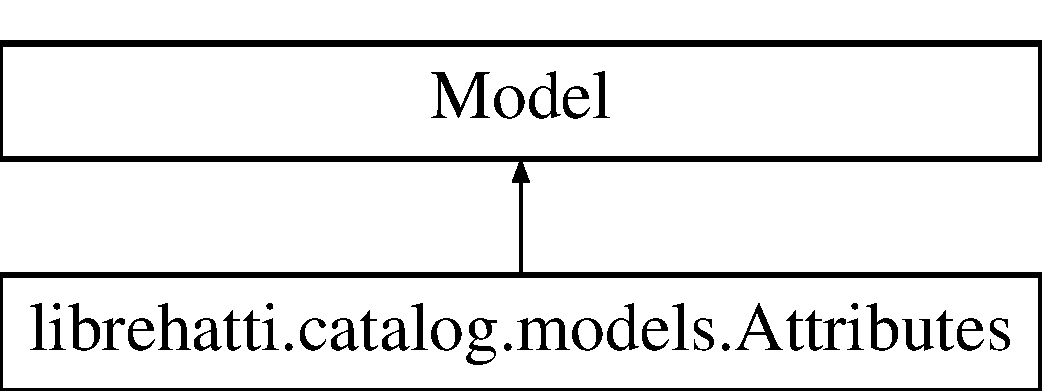
\includegraphics[height=2.000000cm]{classlibrehatti_1_1catalog_1_1models_1_1Attributes}
\end{center}
\end{figure}
\subsection*{Public Member Functions}
\begin{DoxyCompactItemize}
\item 
\hypertarget{classlibrehatti_1_1catalog_1_1models_1_1Attributes_af3990fd5eebcee1d0d19a2b548909a95}{def {\bfseries \-\_\-\-\_\-unicode\-\_\-\-\_\-}}\label{classlibrehatti_1_1catalog_1_1models_1_1Attributes_af3990fd5eebcee1d0d19a2b548909a95}

\end{DoxyCompactItemize}
\subsection*{Static Public Attributes}
\begin{DoxyCompactItemize}
\item 
\hypertarget{classlibrehatti_1_1catalog_1_1models_1_1Attributes_a78c8c34d983715e03c4e4257f543ff50}{tuple {\bfseries name} = models.\-Char\-Field(max\-\_\-length=200)}\label{classlibrehatti_1_1catalog_1_1models_1_1Attributes_a78c8c34d983715e03c4e4257f543ff50}

\item 
\hypertarget{classlibrehatti_1_1catalog_1_1models_1_1Attributes_a6b0c73f5b89a01e105ef1be2cd217b57}{tuple {\bfseries is\-\_\-number} = models.\-Boolean\-Field(default = True)}\label{classlibrehatti_1_1catalog_1_1models_1_1Attributes_a6b0c73f5b89a01e105ef1be2cd217b57}

\item 
\hypertarget{classlibrehatti_1_1catalog_1_1models_1_1Attributes_a29baacb3571048c37b291ee2994336f8}{tuple {\bfseries is\-\_\-string} = models.\-Boolean\-Field(default = False)}\label{classlibrehatti_1_1catalog_1_1models_1_1Attributes_a29baacb3571048c37b291ee2994336f8}

\end{DoxyCompactItemize}


The documentation for this class was generated from the following file\-:\begin{DoxyCompactItemize}
\item 
models.\-py\end{DoxyCompactItemize}

\hypertarget{classlibrehatti_1_1catalog_1_1models_1_1Catalog}{\section{librehatti.\-catalog.\-models.\-Catalog Class Reference}
\label{classlibrehatti_1_1catalog_1_1models_1_1Catalog}\index{librehatti.\-catalog.\-models.\-Catalog@{librehatti.\-catalog.\-models.\-Catalog}}
}
Inheritance diagram for librehatti.\-catalog.\-models.\-Catalog\-:\begin{figure}[H]
\begin{center}
\leavevmode
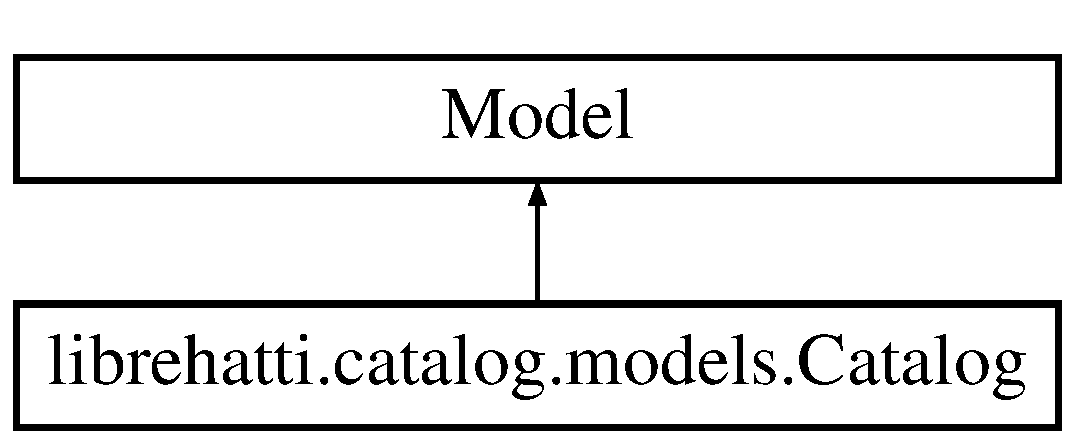
\includegraphics[height=2.000000cm]{classlibrehatti_1_1catalog_1_1models_1_1Catalog}
\end{center}
\end{figure}
\subsection*{Public Member Functions}
\begin{DoxyCompactItemize}
\item 
\hypertarget{classlibrehatti_1_1catalog_1_1models_1_1Catalog_a32caca4cb8a9eeb837b88141eec57105}{def {\bfseries \-\_\-\-\_\-unicode\-\_\-\-\_\-}}\label{classlibrehatti_1_1catalog_1_1models_1_1Catalog_a32caca4cb8a9eeb837b88141eec57105}

\end{DoxyCompactItemize}
\subsection*{Static Public Attributes}
\begin{DoxyCompactItemize}
\item 
\hypertarget{classlibrehatti_1_1catalog_1_1models_1_1Catalog_a5e7e576cafc76d1ae0fdd47bc4655c37}{tuple {\bfseries attribute} = models.\-Foreign\-Key(\hyperlink{classlibrehatti_1_1catalog_1_1models_1_1Attributes}{Attributes})}\label{classlibrehatti_1_1catalog_1_1models_1_1Catalog_a5e7e576cafc76d1ae0fdd47bc4655c37}

\item 
\hypertarget{classlibrehatti_1_1catalog_1_1models_1_1Catalog_a1db0c58938a68db436b6a99aa200f6c4}{tuple {\bfseries value} = models.\-Char\-Field(max\-\_\-length=200)}\label{classlibrehatti_1_1catalog_1_1models_1_1Catalog_a1db0c58938a68db436b6a99aa200f6c4}

\item 
\hypertarget{classlibrehatti_1_1catalog_1_1models_1_1Catalog_a092102657aae060b989cf7eac0f6c7e9}{tuple {\bfseries product} = models.\-Foreign\-Key(\hyperlink{classlibrehatti_1_1catalog_1_1models_1_1Product}{Product})}\label{classlibrehatti_1_1catalog_1_1models_1_1Catalog_a092102657aae060b989cf7eac0f6c7e9}

\end{DoxyCompactItemize}


The documentation for this class was generated from the following file\-:\begin{DoxyCompactItemize}
\item 
models.\-py\end{DoxyCompactItemize}

\hypertarget{classlibrehatti_1_1catalog_1_1admin_1_1CatalogInline}{\section{librehatti.\-catalog.\-admin.\-Catalog\-Inline Class Reference}
\label{classlibrehatti_1_1catalog_1_1admin_1_1CatalogInline}\index{librehatti.\-catalog.\-admin.\-Catalog\-Inline@{librehatti.\-catalog.\-admin.\-Catalog\-Inline}}
}
Inheritance diagram for librehatti.\-catalog.\-admin.\-Catalog\-Inline\-:\begin{figure}[H]
\begin{center}
\leavevmode
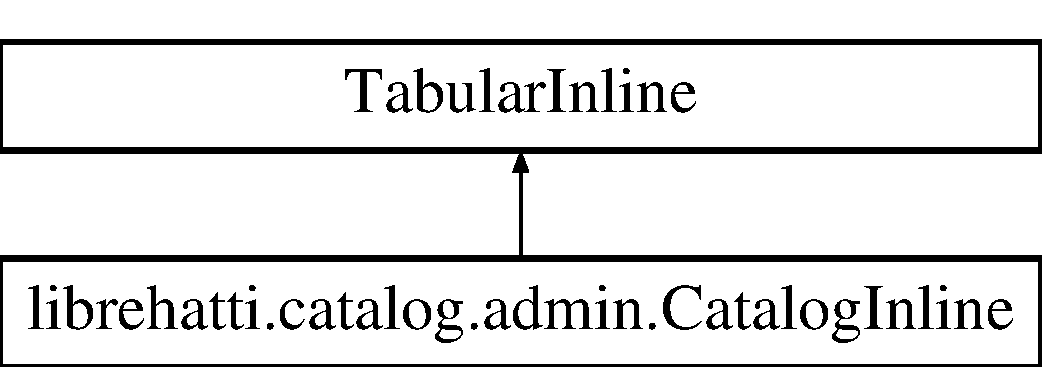
\includegraphics[height=2.000000cm]{classlibrehatti_1_1catalog_1_1admin_1_1CatalogInline}
\end{center}
\end{figure}
\subsection*{Static Public Attributes}
\begin{DoxyCompactItemize}
\item 
\hypertarget{classlibrehatti_1_1catalog_1_1admin_1_1CatalogInline_a788b8a976035dbb1a445475a27aa7587}{{\bfseries model} = \hyperlink{classlibrehatti_1_1catalog_1_1models_1_1Catalog}{Catalog}}\label{classlibrehatti_1_1catalog_1_1admin_1_1CatalogInline_a788b8a976035dbb1a445475a27aa7587}

\item 
\hypertarget{classlibrehatti_1_1catalog_1_1admin_1_1CatalogInline_a365f77bd579f3bbd2d508e96dc1c46c8}{list {\bfseries fields} = \mbox{[}'attribute', 'value'\mbox{]}}\label{classlibrehatti_1_1catalog_1_1admin_1_1CatalogInline_a365f77bd579f3bbd2d508e96dc1c46c8}

\item 
\hypertarget{classlibrehatti_1_1catalog_1_1admin_1_1CatalogInline_a674150452581d0772d76f837688226cd}{int {\bfseries extra} = 10}\label{classlibrehatti_1_1catalog_1_1admin_1_1CatalogInline_a674150452581d0772d76f837688226cd}

\end{DoxyCompactItemize}


The documentation for this class was generated from the following file\-:\begin{DoxyCompactItemize}
\item 
admin.\-py\end{DoxyCompactItemize}

\hypertarget{classlibrehatti_1_1catalog_1_1models_1_1Category}{\section{librehatti.\-catalog.\-models.\-Category Class Reference}
\label{classlibrehatti_1_1catalog_1_1models_1_1Category}\index{librehatti.\-catalog.\-models.\-Category@{librehatti.\-catalog.\-models.\-Category}}
}
Inheritance diagram for librehatti.\-catalog.\-models.\-Category\-:\begin{figure}[H]
\begin{center}
\leavevmode
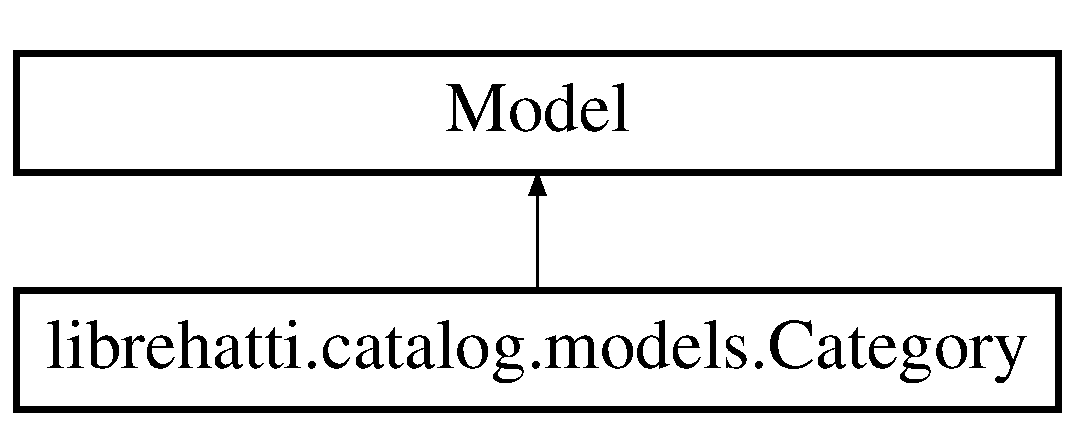
\includegraphics[height=2.000000cm]{classlibrehatti_1_1catalog_1_1models_1_1Category}
\end{center}
\end{figure}
\subsection*{Public Member Functions}
\begin{DoxyCompactItemize}
\item 
\hypertarget{classlibrehatti_1_1catalog_1_1models_1_1Category_a5d88596aaab43cf627cb10fbcddd10e3}{def {\bfseries \-\_\-\-\_\-unicode\-\_\-\-\_\-}}\label{classlibrehatti_1_1catalog_1_1models_1_1Category_a5d88596aaab43cf627cb10fbcddd10e3}

\end{DoxyCompactItemize}
\subsection*{Static Public Attributes}
\begin{DoxyCompactItemize}
\item 
\hypertarget{classlibrehatti_1_1catalog_1_1models_1_1Category_aa4d0431c2037aeb6f7bcca4d110e3206}{tuple {\bfseries name} = models.\-Char\-Field(max\-\_\-length=100)}\label{classlibrehatti_1_1catalog_1_1models_1_1Category_aa4d0431c2037aeb6f7bcca4d110e3206}

\item 
\hypertarget{classlibrehatti_1_1catalog_1_1models_1_1Category_a68ae3d99ee7a2b5b505f76d827a5a87d}{tuple {\bfseries parent} = models.\-Foreign\-Key('self', blank=True, null=True)}\label{classlibrehatti_1_1catalog_1_1models_1_1Category_a68ae3d99ee7a2b5b505f76d827a5a87d}

\end{DoxyCompactItemize}


The documentation for this class was generated from the following file\-:\begin{DoxyCompactItemize}
\item 
models.\-py\end{DoxyCompactItemize}

\hypertarget{classlibrehatti_1_1catalog_1_1models_1_1ModeOfPayment}{\section{librehatti.\-catalog.\-models.\-Mode\-Of\-Payment Class Reference}
\label{classlibrehatti_1_1catalog_1_1models_1_1ModeOfPayment}\index{librehatti.\-catalog.\-models.\-Mode\-Of\-Payment@{librehatti.\-catalog.\-models.\-Mode\-Of\-Payment}}
}
Inheritance diagram for librehatti.\-catalog.\-models.\-Mode\-Of\-Payment\-:\begin{figure}[H]
\begin{center}
\leavevmode
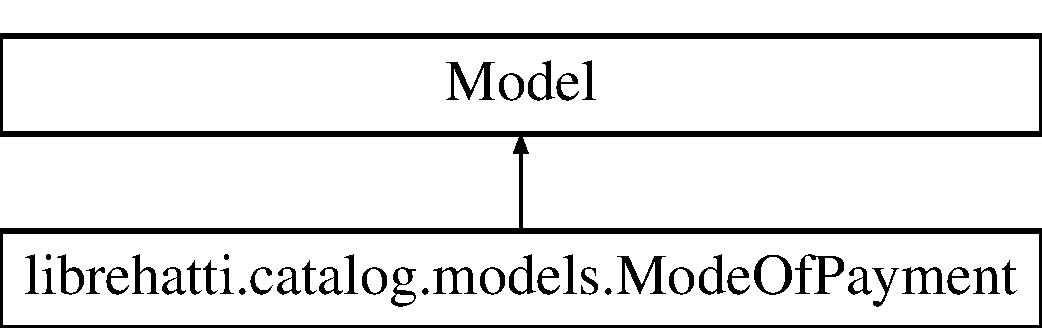
\includegraphics[height=2.000000cm]{classlibrehatti_1_1catalog_1_1models_1_1ModeOfPayment}
\end{center}
\end{figure}
\subsection*{Public Member Functions}
\begin{DoxyCompactItemize}
\item 
\hypertarget{classlibrehatti_1_1catalog_1_1models_1_1ModeOfPayment_ac4474fcac6e4a5f522dce7e071727967}{def {\bfseries \-\_\-\-\_\-unicode\-\_\-\-\_\-}}\label{classlibrehatti_1_1catalog_1_1models_1_1ModeOfPayment_ac4474fcac6e4a5f522dce7e071727967}

\end{DoxyCompactItemize}
\subsection*{Static Public Attributes}
\begin{DoxyCompactItemize}
\item 
\hypertarget{classlibrehatti_1_1catalog_1_1models_1_1ModeOfPayment_ae6576218cba66cc2fc8ea88b6e484dd1}{tuple {\bfseries method} = models.\-Char\-Field(max\-\_\-length=25)}\label{classlibrehatti_1_1catalog_1_1models_1_1ModeOfPayment_ae6576218cba66cc2fc8ea88b6e484dd1}

\end{DoxyCompactItemize}


The documentation for this class was generated from the following file\-:\begin{DoxyCompactItemize}
\item 
models.\-py\end{DoxyCompactItemize}

\hypertarget{classlibrehatti_1_1catalog_1_1models_1_1Product}{\section{librehatti.\-catalog.\-models.\-Product Class Reference}
\label{classlibrehatti_1_1catalog_1_1models_1_1Product}\index{librehatti.\-catalog.\-models.\-Product@{librehatti.\-catalog.\-models.\-Product}}
}
Inheritance diagram for librehatti.\-catalog.\-models.\-Product\-:\begin{figure}[H]
\begin{center}
\leavevmode
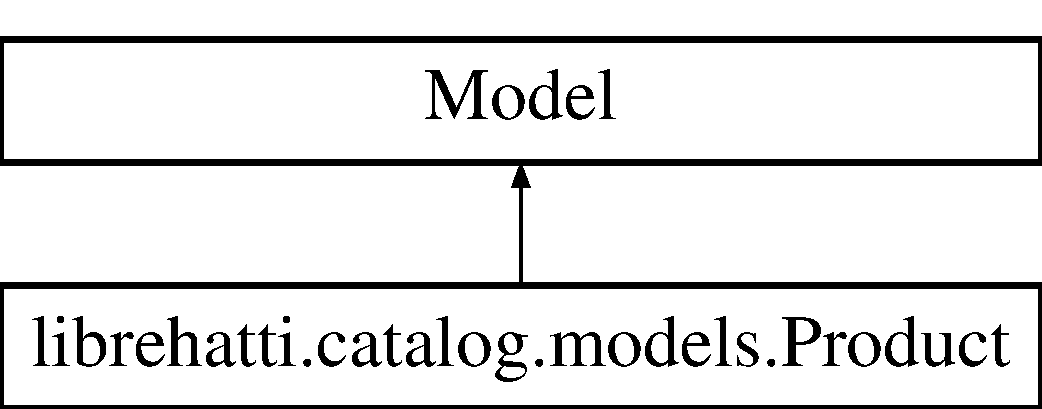
\includegraphics[height=2.000000cm]{classlibrehatti_1_1catalog_1_1models_1_1Product}
\end{center}
\end{figure}
\subsection*{Public Member Functions}
\begin{DoxyCompactItemize}
\item 
\hypertarget{classlibrehatti_1_1catalog_1_1models_1_1Product_a91388ae14c28db01a8a1bc32edb90d87}{def {\bfseries \-\_\-\-\_\-unicode\-\_\-\-\_\-}}\label{classlibrehatti_1_1catalog_1_1models_1_1Product_a91388ae14c28db01a8a1bc32edb90d87}

\end{DoxyCompactItemize}
\subsection*{Static Public Attributes}
\begin{DoxyCompactItemize}
\item 
\hypertarget{classlibrehatti_1_1catalog_1_1models_1_1Product_aa001ecb05e4ad78d3438351cd1ad70fd}{tuple {\bfseries name} = models.\-Char\-Field(max\-\_\-length=100)}\label{classlibrehatti_1_1catalog_1_1models_1_1Product_aa001ecb05e4ad78d3438351cd1ad70fd}

\item 
\hypertarget{classlibrehatti_1_1catalog_1_1models_1_1Product_a1125cc90bcd74b53e19efb82d32305d0}{tuple {\bfseries category} = models.\-Foreign\-Key(\hyperlink{classlibrehatti_1_1catalog_1_1models_1_1Category}{Category})}\label{classlibrehatti_1_1catalog_1_1models_1_1Product_a1125cc90bcd74b53e19efb82d32305d0}

\item 
\hypertarget{classlibrehatti_1_1catalog_1_1models_1_1Product_a75c525f7f2cd2fb250c59fe29c28debc}{tuple {\bfseries price\-\_\-per\-\_\-unit} = models.\-Integer\-Field()}\label{classlibrehatti_1_1catalog_1_1models_1_1Product_a75c525f7f2cd2fb250c59fe29c28debc}

\item 
\hypertarget{classlibrehatti_1_1catalog_1_1models_1_1Product_a30c965e403d19f8a328e4e990b4fddff}{tuple {\bfseries organisation} = models.\-Foreign\-Key('useraccounts.\-Admin\-Organisations')}\label{classlibrehatti_1_1catalog_1_1models_1_1Product_a30c965e403d19f8a328e4e990b4fddff}

\end{DoxyCompactItemize}


The documentation for this class was generated from the following file\-:\begin{DoxyCompactItemize}
\item 
models.\-py\end{DoxyCompactItemize}

\hypertarget{classlibrehatti_1_1catalog_1_1admin_1_1ProductAdmin}{\section{librehatti.\-catalog.\-admin.\-Product\-Admin Class Reference}
\label{classlibrehatti_1_1catalog_1_1admin_1_1ProductAdmin}\index{librehatti.\-catalog.\-admin.\-Product\-Admin@{librehatti.\-catalog.\-admin.\-Product\-Admin}}
}
Inheritance diagram for librehatti.\-catalog.\-admin.\-Product\-Admin\-:\begin{figure}[H]
\begin{center}
\leavevmode
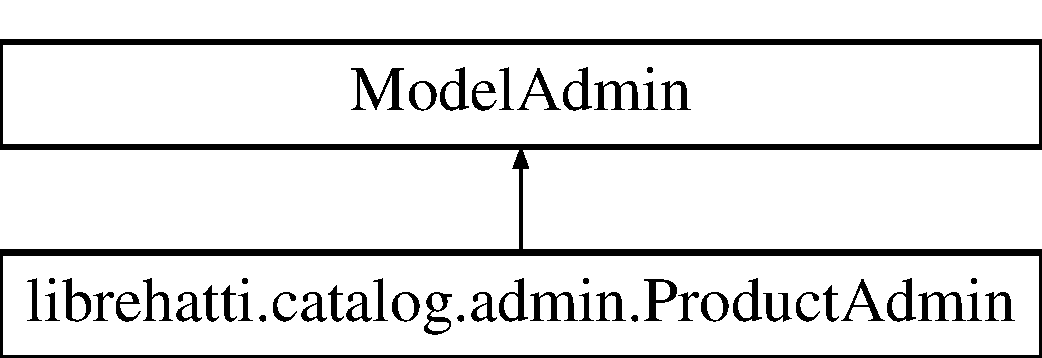
\includegraphics[height=2.000000cm]{classlibrehatti_1_1catalog_1_1admin_1_1ProductAdmin}
\end{center}
\end{figure}
\subsection*{Static Public Attributes}
\begin{DoxyCompactItemize}
\item 
\hypertarget{classlibrehatti_1_1catalog_1_1admin_1_1ProductAdmin_a3bfaf5e99f9f0f095224b36bd0244280}{list {\bfseries fields} = \mbox{[}'name', 'category', 'price\-\_\-per\-\_\-unit', 'organisation'\mbox{]}}\label{classlibrehatti_1_1catalog_1_1admin_1_1ProductAdmin_a3bfaf5e99f9f0f095224b36bd0244280}

\item 
\hypertarget{classlibrehatti_1_1catalog_1_1admin_1_1ProductAdmin_a68b23952630280d1a8f19d7da02cea0c}{list {\bfseries inlines} = \mbox{[}\hyperlink{classlibrehatti_1_1catalog_1_1admin_1_1CatalogInline}{Catalog\-Inline}\mbox{]}}\label{classlibrehatti_1_1catalog_1_1admin_1_1ProductAdmin_a68b23952630280d1a8f19d7da02cea0c}

\end{DoxyCompactItemize}


The documentation for this class was generated from the following file\-:\begin{DoxyCompactItemize}
\item 
admin.\-py\end{DoxyCompactItemize}

\hypertarget{classlibrehatti_1_1catalog_1_1models_1_1PurchasedItem}{\section{librehatti.\-catalog.\-models.\-Purchased\-Item Class Reference}
\label{classlibrehatti_1_1catalog_1_1models_1_1PurchasedItem}\index{librehatti.\-catalog.\-models.\-Purchased\-Item@{librehatti.\-catalog.\-models.\-Purchased\-Item}}
}
Inheritance diagram for librehatti.\-catalog.\-models.\-Purchased\-Item\-:\begin{figure}[H]
\begin{center}
\leavevmode
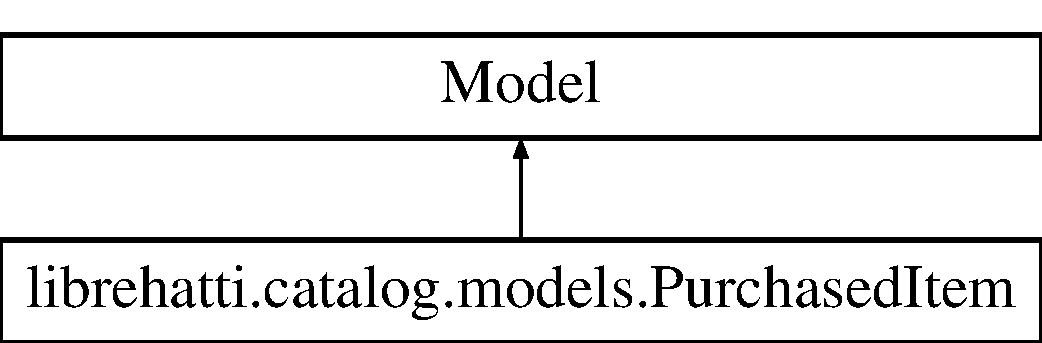
\includegraphics[height=2.000000cm]{classlibrehatti_1_1catalog_1_1models_1_1PurchasedItem}
\end{center}
\end{figure}
\subsection*{Public Member Functions}
\begin{DoxyCompactItemize}
\item 
\hypertarget{classlibrehatti_1_1catalog_1_1models_1_1PurchasedItem_a166fc847aabefa7daf910abd24d2d3af}{def {\bfseries save}}\label{classlibrehatti_1_1catalog_1_1models_1_1PurchasedItem_a166fc847aabefa7daf910abd24d2d3af}

\item 
\hypertarget{classlibrehatti_1_1catalog_1_1models_1_1PurchasedItem_abf536261b59c1b8c155619f960e179fd}{def {\bfseries \-\_\-\-\_\-unicode\-\_\-\-\_\-}}\label{classlibrehatti_1_1catalog_1_1models_1_1PurchasedItem_abf536261b59c1b8c155619f960e179fd}

\end{DoxyCompactItemize}
\subsection*{Public Attributes}
\begin{DoxyCompactItemize}
\item 
\hypertarget{classlibrehatti_1_1catalog_1_1models_1_1PurchasedItem_a4501d413b89ac16cc15225cd8aa63045}{{\bfseries price}}\label{classlibrehatti_1_1catalog_1_1models_1_1PurchasedItem_a4501d413b89ac16cc15225cd8aa63045}

\end{DoxyCompactItemize}
\subsection*{Static Public Attributes}
\begin{DoxyCompactItemize}
\item 
\hypertarget{classlibrehatti_1_1catalog_1_1models_1_1PurchasedItem_a99aef17e99c9046543539eb9f45aa838}{tuple {\bfseries purchase\-\_\-order} = models.\-Foreign\-Key(\hyperlink{classlibrehatti_1_1catalog_1_1models_1_1PurchaseOrder}{Purchase\-Order})}\label{classlibrehatti_1_1catalog_1_1models_1_1PurchasedItem_a99aef17e99c9046543539eb9f45aa838}

\item 
\hypertarget{classlibrehatti_1_1catalog_1_1models_1_1PurchasedItem_a1db422be2bd4bc3d775ab8021755d200}{tuple {\bfseries price} = models.\-Integer\-Field()}\label{classlibrehatti_1_1catalog_1_1models_1_1PurchasedItem_a1db422be2bd4bc3d775ab8021755d200}

\item 
\hypertarget{classlibrehatti_1_1catalog_1_1models_1_1PurchasedItem_a9708cbe064d626b30eabcb2e2b3c7439}{tuple {\bfseries qty} = models.\-Integer\-Field()}\label{classlibrehatti_1_1catalog_1_1models_1_1PurchasedItem_a9708cbe064d626b30eabcb2e2b3c7439}

\item 
\hypertarget{classlibrehatti_1_1catalog_1_1models_1_1PurchasedItem_aa7832d5850ead70256725c310883e8d8}{tuple {\bfseries item} = models.\-Foreign\-Key(\hyperlink{classlibrehatti_1_1catalog_1_1models_1_1Product}{Product})}\label{classlibrehatti_1_1catalog_1_1models_1_1PurchasedItem_aa7832d5850ead70256725c310883e8d8}

\end{DoxyCompactItemize}


The documentation for this class was generated from the following file\-:\begin{DoxyCompactItemize}
\item 
models.\-py\end{DoxyCompactItemize}

\hypertarget{classlibrehatti_1_1catalog_1_1admin_1_1PurchasedItemInline}{\section{librehatti.\-catalog.\-admin.\-Purchased\-Item\-Inline Class Reference}
\label{classlibrehatti_1_1catalog_1_1admin_1_1PurchasedItemInline}\index{librehatti.\-catalog.\-admin.\-Purchased\-Item\-Inline@{librehatti.\-catalog.\-admin.\-Purchased\-Item\-Inline}}
}
Inheritance diagram for librehatti.\-catalog.\-admin.\-Purchased\-Item\-Inline\-:\begin{figure}[H]
\begin{center}
\leavevmode
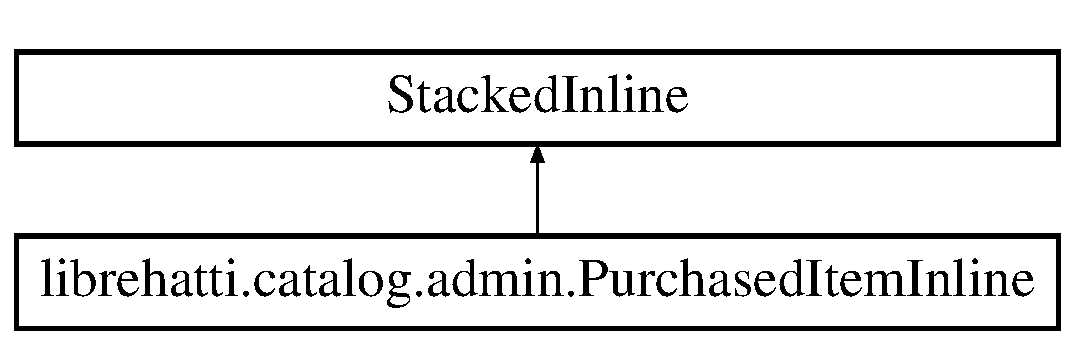
\includegraphics[height=2.000000cm]{classlibrehatti_1_1catalog_1_1admin_1_1PurchasedItemInline}
\end{center}
\end{figure}
\subsection*{Static Public Attributes}
\begin{DoxyCompactItemize}
\item 
\hypertarget{classlibrehatti_1_1catalog_1_1admin_1_1PurchasedItemInline_a7c61aeec8b94ca50e53c9c341ad8fca8}{{\bfseries model} = \hyperlink{classlibrehatti_1_1catalog_1_1models_1_1PurchasedItem}{Purchased\-Item}}\label{classlibrehatti_1_1catalog_1_1admin_1_1PurchasedItemInline_a7c61aeec8b94ca50e53c9c341ad8fca8}

\item 
\hypertarget{classlibrehatti_1_1catalog_1_1admin_1_1PurchasedItemInline_a05deeded81a6a9daab5823eccce84df5}{list {\bfseries fields} = \mbox{[}'item', 'qty', \mbox{]}}\label{classlibrehatti_1_1catalog_1_1admin_1_1PurchasedItemInline_a05deeded81a6a9daab5823eccce84df5}

\item 
\hypertarget{classlibrehatti_1_1catalog_1_1admin_1_1PurchasedItemInline_ae7c4b7ddbc9841c10fc7aa7ae8a5c6c0}{int {\bfseries extra} = 10}\label{classlibrehatti_1_1catalog_1_1admin_1_1PurchasedItemInline_ae7c4b7ddbc9841c10fc7aa7ae8a5c6c0}

\end{DoxyCompactItemize}


The documentation for this class was generated from the following file\-:\begin{DoxyCompactItemize}
\item 
admin.\-py\end{DoxyCompactItemize}

\hypertarget{classlibrehatti_1_1catalog_1_1models_1_1PurchaseOrder}{\section{librehatti.\-catalog.\-models.\-Purchase\-Order Class Reference}
\label{classlibrehatti_1_1catalog_1_1models_1_1PurchaseOrder}\index{librehatti.\-catalog.\-models.\-Purchase\-Order@{librehatti.\-catalog.\-models.\-Purchase\-Order}}
}
Inheritance diagram for librehatti.\-catalog.\-models.\-Purchase\-Order\-:\begin{figure}[H]
\begin{center}
\leavevmode
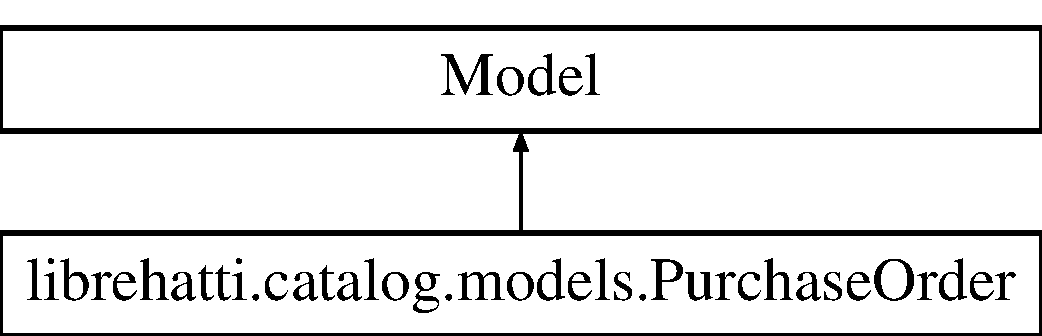
\includegraphics[height=2.000000cm]{classlibrehatti_1_1catalog_1_1models_1_1PurchaseOrder}
\end{center}
\end{figure}
\subsection*{Public Member Functions}
\begin{DoxyCompactItemize}
\item 
\hypertarget{classlibrehatti_1_1catalog_1_1models_1_1PurchaseOrder_aabe49ee20451298a11e44e2474872fb0}{def {\bfseries \-\_\-\-\_\-unicode\-\_\-\-\_\-}}\label{classlibrehatti_1_1catalog_1_1models_1_1PurchaseOrder_aabe49ee20451298a11e44e2474872fb0}

\end{DoxyCompactItemize}
\subsection*{Static Public Attributes}
\begin{DoxyCompactItemize}
\item 
\hypertarget{classlibrehatti_1_1catalog_1_1models_1_1PurchaseOrder_a2768a892466a2be1f40b05ab7d4d6d56}{tuple {\bfseries buyer\-\_\-id} = models.\-Foreign\-Key(User)}\label{classlibrehatti_1_1catalog_1_1models_1_1PurchaseOrder_a2768a892466a2be1f40b05ab7d4d6d56}

\item 
\hypertarget{classlibrehatti_1_1catalog_1_1models_1_1PurchaseOrder_abe0c5fe56c845603360c5c0b27885337}{tuple {\bfseries is\-\_\-debit} = models.\-Boolean\-Field(default = False)}\label{classlibrehatti_1_1catalog_1_1models_1_1PurchaseOrder_abe0c5fe56c845603360c5c0b27885337}

\item 
\hypertarget{classlibrehatti_1_1catalog_1_1models_1_1PurchaseOrder_a906409ea32a270b2d2aa9c4cef6919e2}{tuple {\bfseries delivery\-\_\-address} = models.\-Foreign\-Key('useraccounts.\-Address')}\label{classlibrehatti_1_1catalog_1_1models_1_1PurchaseOrder_a906409ea32a270b2d2aa9c4cef6919e2}

\item 
\hypertarget{classlibrehatti_1_1catalog_1_1models_1_1PurchaseOrder_aa8ad9c440b1993397b7189f58d878fd0}{tuple {\bfseries organisation} = models.\-Foreign\-Key('useraccounts.\-Admin\-Organisations')}\label{classlibrehatti_1_1catalog_1_1models_1_1PurchaseOrder_aa8ad9c440b1993397b7189f58d878fd0}

\item 
\hypertarget{classlibrehatti_1_1catalog_1_1models_1_1PurchaseOrder_abd767c1140af50d0ce7e5f0229cfaa17}{tuple {\bfseries date\-\_\-time} = models.\-Date\-Time\-Field(auto\-\_\-now\-\_\-add=True)}\label{classlibrehatti_1_1catalog_1_1models_1_1PurchaseOrder_abd767c1140af50d0ce7e5f0229cfaa17}

\item 
\hypertarget{classlibrehatti_1_1catalog_1_1models_1_1PurchaseOrder_abb45b6bc4b47e0563a020ebd64aaa173}{tuple {\bfseries total\-\_\-discount} = models.\-Integer\-Field()}\label{classlibrehatti_1_1catalog_1_1models_1_1PurchaseOrder_abb45b6bc4b47e0563a020ebd64aaa173}

\item 
\hypertarget{classlibrehatti_1_1catalog_1_1models_1_1PurchaseOrder_a2666468af212f2b0e606dec24b6f0edd}{tuple {\bfseries tds} = models.\-Integer\-Field()}\label{classlibrehatti_1_1catalog_1_1models_1_1PurchaseOrder_a2666468af212f2b0e606dec24b6f0edd}

\item 
\hypertarget{classlibrehatti_1_1catalog_1_1models_1_1PurchaseOrder_ad331d566b7b412ad4ac420e7ea6cd931}{tuple {\bfseries mode\-\_\-of\-\_\-payment} = models.\-Foreign\-Key(\hyperlink{classlibrehatti_1_1catalog_1_1models_1_1ModeOfPayment}{Mode\-Of\-Payment})}\label{classlibrehatti_1_1catalog_1_1models_1_1PurchaseOrder_ad331d566b7b412ad4ac420e7ea6cd931}

\end{DoxyCompactItemize}


The documentation for this class was generated from the following file\-:\begin{DoxyCompactItemize}
\item 
models.\-py\end{DoxyCompactItemize}

\hypertarget{classlibrehatti_1_1catalog_1_1admin_1_1PurchaseOrderAdmin}{\section{librehatti.\-catalog.\-admin.\-Purchase\-Order\-Admin Class Reference}
\label{classlibrehatti_1_1catalog_1_1admin_1_1PurchaseOrderAdmin}\index{librehatti.\-catalog.\-admin.\-Purchase\-Order\-Admin@{librehatti.\-catalog.\-admin.\-Purchase\-Order\-Admin}}
}
Inheritance diagram for librehatti.\-catalog.\-admin.\-Purchase\-Order\-Admin\-:\begin{figure}[H]
\begin{center}
\leavevmode
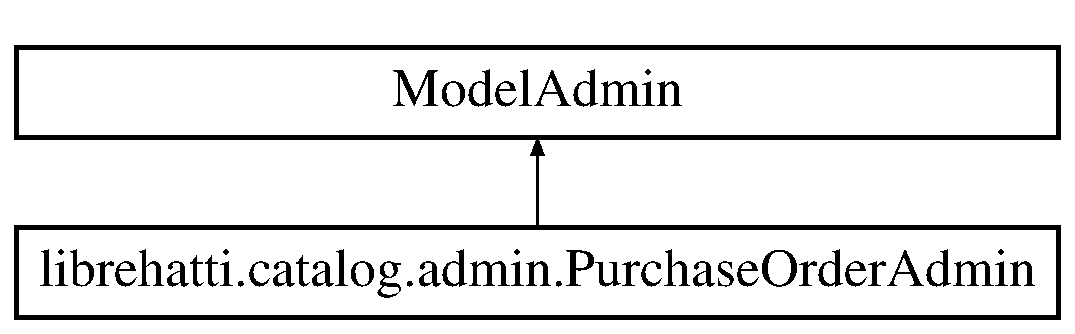
\includegraphics[height=2.000000cm]{classlibrehatti_1_1catalog_1_1admin_1_1PurchaseOrderAdmin}
\end{center}
\end{figure}
\subsection*{Public Member Functions}
\begin{DoxyCompactItemize}
\item 
\hypertarget{classlibrehatti_1_1catalog_1_1admin_1_1PurchaseOrderAdmin_a8033956ae850614346e5513658c243b3}{def {\bfseries response\-\_\-add}}\label{classlibrehatti_1_1catalog_1_1admin_1_1PurchaseOrderAdmin_a8033956ae850614346e5513658c243b3}

\end{DoxyCompactItemize}
\subsection*{Static Public Attributes}
\begin{DoxyCompactItemize}
\item 
\hypertarget{classlibrehatti_1_1catalog_1_1admin_1_1PurchaseOrderAdmin_a9926cfc46cacd53a08960127eec229e7}{tuple {\bfseries exclude} = ('is\-\_\-suspense',)}\label{classlibrehatti_1_1catalog_1_1admin_1_1PurchaseOrderAdmin_a9926cfc46cacd53a08960127eec229e7}

\item 
\hypertarget{classlibrehatti_1_1catalog_1_1admin_1_1PurchaseOrderAdmin_a0c31c8d7ad03fb4308293b169f849b98}{list {\bfseries inlines} = \mbox{[}\hyperlink{classlibrehatti_1_1catalog_1_1admin_1_1PurchasedItemInline}{Purchased\-Item\-Inline}\mbox{]}}\label{classlibrehatti_1_1catalog_1_1admin_1_1PurchaseOrderAdmin_a0c31c8d7ad03fb4308293b169f849b98}

\item 
\hypertarget{classlibrehatti_1_1catalog_1_1admin_1_1PurchaseOrderAdmin_aaac78c87d4a7687aa030d32ab8809443}{{\bfseries model} = \hyperlink{classlibrehatti_1_1catalog_1_1models_1_1PurchaseOrder}{Purchase\-Order}}\label{classlibrehatti_1_1catalog_1_1admin_1_1PurchaseOrderAdmin_aaac78c87d4a7687aa030d32ab8809443}

\end{DoxyCompactItemize}


The documentation for this class was generated from the following file\-:\begin{DoxyCompactItemize}
\item 
admin.\-py\end{DoxyCompactItemize}

\hypertarget{classlibrehatti_1_1catalog_1_1tests_1_1SimpleTest}{\section{librehatti.\-catalog.\-tests.\-Simple\-Test Class Reference}
\label{classlibrehatti_1_1catalog_1_1tests_1_1SimpleTest}\index{librehatti.\-catalog.\-tests.\-Simple\-Test@{librehatti.\-catalog.\-tests.\-Simple\-Test}}
}
Inheritance diagram for librehatti.\-catalog.\-tests.\-Simple\-Test\-:\begin{figure}[H]
\begin{center}
\leavevmode
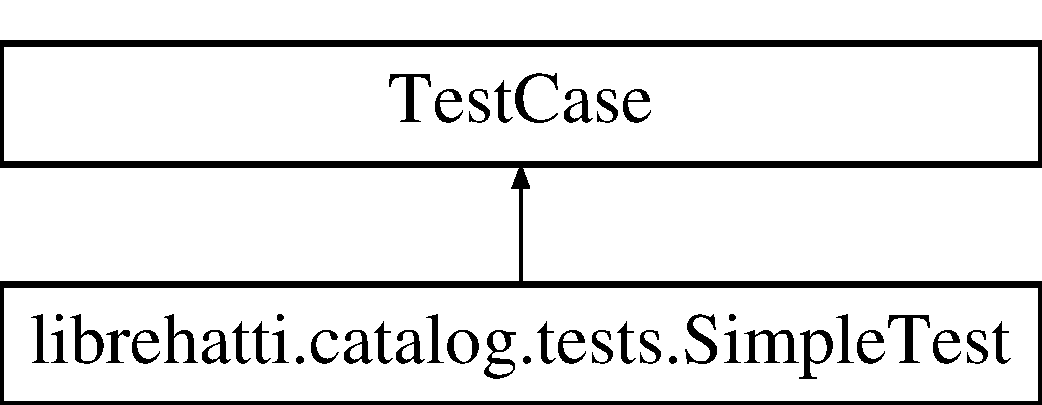
\includegraphics[height=2.000000cm]{classlibrehatti_1_1catalog_1_1tests_1_1SimpleTest}
\end{center}
\end{figure}
\subsection*{Public Member Functions}
\begin{DoxyCompactItemize}
\item 
\hypertarget{classlibrehatti_1_1catalog_1_1tests_1_1SimpleTest_a2850a4dc6ec1017ac441eb59f9d7d5ad}{def {\bfseries test\-\_\-basic\-\_\-addition}}\label{classlibrehatti_1_1catalog_1_1tests_1_1SimpleTest_a2850a4dc6ec1017ac441eb59f9d7d5ad}

\end{DoxyCompactItemize}


The documentation for this class was generated from the following file\-:\begin{DoxyCompactItemize}
\item 
tests.\-py\end{DoxyCompactItemize}

\hypertarget{classlibrehatti_1_1catalog_1_1models_1_1Surcharge}{\section{librehatti.\-catalog.\-models.\-Surcharge Class Reference}
\label{classlibrehatti_1_1catalog_1_1models_1_1Surcharge}\index{librehatti.\-catalog.\-models.\-Surcharge@{librehatti.\-catalog.\-models.\-Surcharge}}
}
Inheritance diagram for librehatti.\-catalog.\-models.\-Surcharge\-:\begin{figure}[H]
\begin{center}
\leavevmode
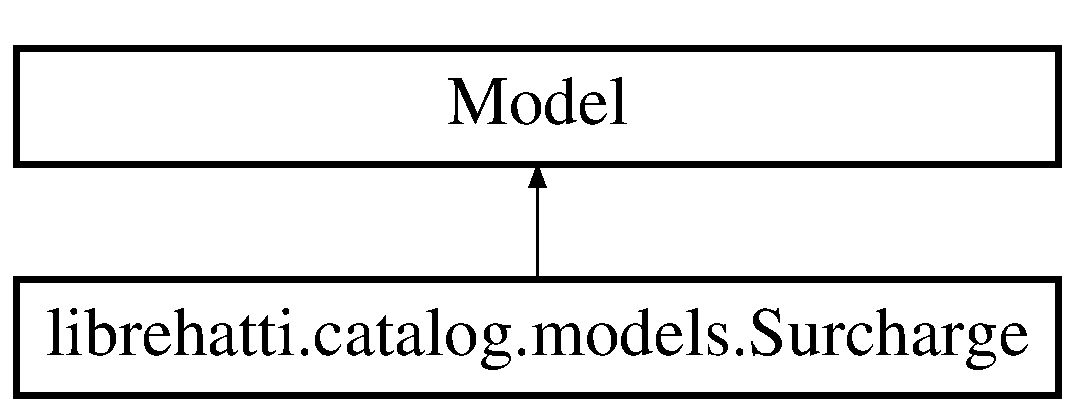
\includegraphics[height=2.000000cm]{classlibrehatti_1_1catalog_1_1models_1_1Surcharge}
\end{center}
\end{figure}
\subsection*{Public Member Functions}
\begin{DoxyCompactItemize}
\item 
\hypertarget{classlibrehatti_1_1catalog_1_1models_1_1Surcharge_a2fe3f353f5eb8b481865133d25acfcec}{def {\bfseries \-\_\-\-\_\-unicode\-\_\-\-\_\-}}\label{classlibrehatti_1_1catalog_1_1models_1_1Surcharge_a2fe3f353f5eb8b481865133d25acfcec}

\end{DoxyCompactItemize}
\subsection*{Static Public Attributes}
\begin{DoxyCompactItemize}
\item 
\hypertarget{classlibrehatti_1_1catalog_1_1models_1_1Surcharge_adaabe9567e606abaa08e7b653e4a08dc}{tuple {\bfseries taxes} = models.\-Char\-Field(max\-\_\-length=200)}\label{classlibrehatti_1_1catalog_1_1models_1_1Surcharge_adaabe9567e606abaa08e7b653e4a08dc}

\item 
\hypertarget{classlibrehatti_1_1catalog_1_1models_1_1Surcharge_a6a0a37261bf13ac475141f7a7d946949}{tuple {\bfseries value} = models.\-Integer\-Field()}\label{classlibrehatti_1_1catalog_1_1models_1_1Surcharge_a6a0a37261bf13ac475141f7a7d946949}

\item 
\hypertarget{classlibrehatti_1_1catalog_1_1models_1_1Surcharge_a6c3521bf9e35f0d60ddcca887b0682f0}{tuple {\bfseries taxes\-\_\-included} = models.\-Boolean\-Field(default = False)}\label{classlibrehatti_1_1catalog_1_1models_1_1Surcharge_a6c3521bf9e35f0d60ddcca887b0682f0}

\item 
\hypertarget{classlibrehatti_1_1catalog_1_1models_1_1Surcharge_a11bc15d4fbe997aa74ef349d3b76bffa}{tuple {\bfseries tax\-\_\-effected\-\_\-from} = models.\-Date\-Field()}\label{classlibrehatti_1_1catalog_1_1models_1_1Surcharge_a11bc15d4fbe997aa74ef349d3b76bffa}

\item 
\hypertarget{classlibrehatti_1_1catalog_1_1models_1_1Surcharge_a024bd9f4db5f87b1c8678aaecde0943e}{tuple {\bfseries tax\-\_\-valid\-\_\-till} = models.\-Date\-Field()}\label{classlibrehatti_1_1catalog_1_1models_1_1Surcharge_a024bd9f4db5f87b1c8678aaecde0943e}

\item 
\hypertarget{classlibrehatti_1_1catalog_1_1models_1_1Surcharge_a8406404e2369d4e81a89a1bed75a9807}{tuple {\bfseries Remark} = models.\-Char\-Field(max\-\_\-length=1000)}\label{classlibrehatti_1_1catalog_1_1models_1_1Surcharge_a8406404e2369d4e81a89a1bed75a9807}

\end{DoxyCompactItemize}


The documentation for this class was generated from the following file\-:\begin{DoxyCompactItemize}
\item 
models.\-py\end{DoxyCompactItemize}

%--- End generated contents ---

% Index
\newpage
\phantomsection
\addcontentsline{toc}{chapter}{Index}
\printindex

\end{document}
